\documentclass{beamer}
\usepackage[utf8]{inputenc}
\usepackage[english]{babel}
\usepackage[T1]{fontenc}
\usepackage[inline]{asymptote}
\usepackage{pgfplots}
\pgfplotsset{compat=1.5} 
\usepgfplotslibrary{statistics}
\usepackage{slide_helper}

\title[MA205 - Section 3.2]{Measures of Variation}

\newcommand{\textsep}{\vspace{0.5mm}}

\begin{document}
\begin{frame}
\titlepage
\end{frame}

\begin{frame}[fragile]
\begin{example}
Consider the dotplot of waiting times at a bank.
\begin{center}
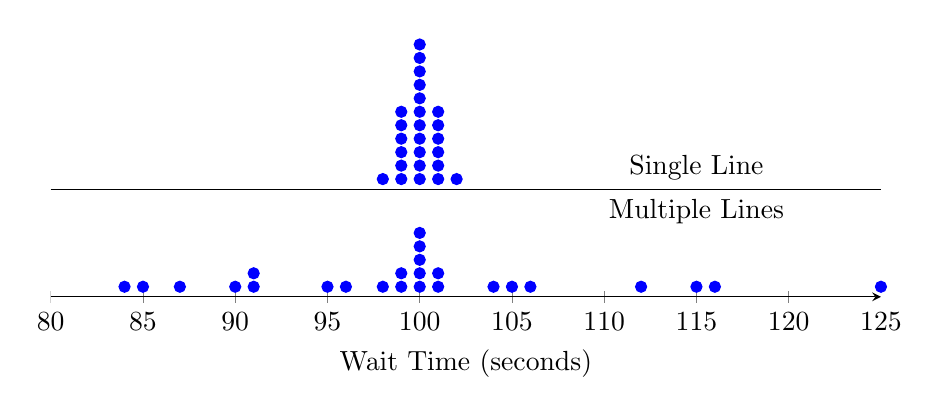
\begin{tikzpicture}
\begin{axis}[
width=\linewidth,
height=5cm,
xlabel={Wait Time (seconds)},
ylabel={},
yticklabels={},
axis y line=none,
axis x line=bottom,
ymin=0,
ymax=20,
xmin=80,
xmax=125,
scatter/use mapped color={
 %draw=mapped color,
 fill=blue,
},
]
\addplot[scatter, only marks, blue, scatter src=y]
coordinates
{
(84, 0.75)
(85, 0.75)
(87, 0.75)
(90, 0.75)
(91, 0.75)
(91, 1.75)
(95, 0.75)
(96, 0.75)
(98, 0.75)
(99, 0.75)
(99, 1.75)
(100, 0.75)
(100, 1.75)
(100, 2.75)
(100, 3.75)
(100, 4.75)
(101, 0.75)
(101, 1.75)
(104, 0.75)
(105, 0.75)
(106, 0.75)
(112, 0.75)
(115, 0.75)
(116, 0.75)
(125, 0.75)
};

\draw (axis cs:80,8) -- (axis cs:125,8);
\draw (axis cs:115,8) node[above]{Single Line};
\draw (axis cs:115,8) node[below]{Multiple Lines};

\addplot[scatter, only marks, blue, scatter src=y]
coordinates
{
(98, 8.75)
(99, 8.75)
(99, 9.75)
(99, 10.75)
(99, 11.75)
(99, 12.75)
(99, 13.75)
(100, 8.75)
(100, 9.75)
(100, 10.75)
(100, 11.75)
(100, 12.75)
(100, 13.75)
(100, 14.75)
(100, 15.75)
(100, 16.75)
(100, 17.75)
(100, 18.75)
(101, 8.75)
(101, 9.75)
(101, 10.75)
(101, 11.75)
(101, 12.75)
(101, 13.75)
(102, 8.75)
};
\end{axis}
\end{tikzpicture}
\end{center}\pause

Both of these data sets have the same mean, but there are clearly different.\pause

\vspace{2mm}
The bank didn't switch to multiple lines because it made them more efficient, nor because customer wait times were reduced, but because customers prefer waiting times with less variation.
\end{example}
\end{frame}

\begin{frame}
\begin{definition}
The \textbf{range} of a set of data values is the difference between the maximum data value and the minimum data value.
\begin{equation*}
\text{Range} = (\text{maximum data value})-(\text{minimum data value})
\end{equation*}
\end{definition}\pause

\begin{block}{Properties}
\begin{itemize}
\item The range is very sensitive to extreme values.\pause
\item Because the range only uses two values it does not reflect the true variation among all of the data values.
\end{itemize}
\end{block}
\end{frame}

\begin{frame}
\begin{example}
Data set 32 \textquote{Airport Data Speeds} in Appendix B includes measures of data speeds of smartphones from four different carriers. The table contains five data speeds, in megabits per second (Mbps), from the data set.

\begin{center}
\begin{tabular}{|l|ccccc|}\hline
\text{Verizon} & 38.5 & \textcolor<2->{blue}{55.6} & 22.4 & \textcolor<2->{red}{14.1} & 23.1\\\hline
\end{tabular}
\end{center}\pause

The range is
\begin{equation*}
\text{Range} = \textcolor{blue}{55.6}-\textcolor{red}{14.1}\pause
= 41.50~\text{Mbps}
\end{equation*}
\end{example}
\end{frame}

\end{document}
